{\noindent \normalsize \bf Dear VLDB Chairs and Referees: }

\vspace{.5em}

We thank the reviewers and chair for the helpful feedback on our paper. 
We addressed all of the concerns and included references to the revised text. 
To remind the reviewers, \sys is a model training framework that allows for iterative data cleaning with provable convergence properties.
\sys presents a number of optimizations to adaptively select records to clean that are likely to be dirty and those that are most valuable to the model.
In summary, the major revisions are:

\begin{enumerate}
\item We include new experimental results on a real dataset of movie plot descriptions from IMDB with real data error, and also clarify that the experiment that was previously in the paper was real as well~(Section \label{real-errors}). Accordingly, we have re-organized the experiments section to describe these real uses in more detail.

\item As the reviewers suggested, we have revised Section \ref{intro} and Section \ref{background} to introduce the problem of interactive data cleaning and model training. We expanded our discussion about the convergence problem in the introduction, and revised our background section to illustrate this problem in the context of one of our experimental datasets.

\item We further revised the presentation of the sampling component of \sys. By ``sampling'', we mean that in each iteration \sys selects new data to be cleaned but this has to be done stochastically to avoid introducing biases. We clarify that this does not mean that the data are sampled up-front as in~\cite{wang1999sample}.

\item We have also clarified the relationship between \sys and Active Learning. Active Learning studies the problem of acquiring the most valuable labels for unlabeled data. On the other hand, \sys studies select the most valuable data to clean in a dirty dataset. \sys modifies both the features and the labels.

\end{enumerate}

\subsection*{Meta Review Details} 

\noindent\noindent \textbf{This paper addresses an interesting problem: interactively cleaning data to improve ML models. Reviewers are happy with the theoretical results on convergence and the solution proposed. One important concern is the lack of experiments on real dirty data. Hopefully this can be addressed in a revision.}

\vspace{0.5em}

We thank the reviewers for insisting on an evaluation of \sys on a real dataset. We believe that benchmarking data cleaning techniques on real use cases is an important problem, and accordingly, we have revised our experiments (Section \ref{eval}) to include a result on a real dataset with real errors. 

This scenario explores a dataset of movie descriptions scrapped from the Internet Movie Database (IMDB). 
Each movie has a title, a 1-2 paragraph plot description, and a list of categories.
We want to train a classification model that predicts whether a movie is a ``Horror'' movie or a ``Comedy'' from the plot description and the title.
However, since much of this data is user contributed, the category listd are often dirty with redundant and sometimes conflicting tags.
Furthermore, there are numerous examples of parsing artifacts in the plot description.
We clean this dataset by cross-referencing the IMDB dataset with a cleaner, curated dataset of movies from Yahoo.

This dataset also shows experimental evidence for systematic bias in the data error.
Horror movies were more likely to be erroneously tagged. 
On the dirty dataset, the prediction precision of the classification model for Horror movies was only 29\%.
This improved to 74\% after data cleaning.

In our original submission, we did include an experiment performed on real data with real errors. 
We apologize that the writing was unclear. We have revised the experiments to move the real datasets up-front~\cite{real-errors}, and expanded our discussion about the datasets, challenges, and results.

\subsection*{Review 1 Details} 

\noindent\textbf{R1.1: I'm not fully convinced that mixed dirty and clean data can be even worse than no cleaning. It would be helpful to show experimental support from the beginning for this and clarify whether this holds in general or only applies to certain models.}

\noindent We have updated the introduction, background, and experiments to better emphasize that training on a mix of dirty and clean data can have misleading result.
The introduction 
The basic problem is that any aggregate over multiple populations of data is susceptible to a bias called Simpson's Paradox. 
This problem has affected a number of high-profile studies outside of the context of data cleaning (e.g.,~\cite{bickel1975sex, charig1986comparison}. 
In the introduction and background sections, we clarify how this statistical problem is relevant to data cleaning and model training since partial cleaning creates two populations of data. 
Even if this approach sometimes works, we argue that it is incorrect in general.
Experiments in Section \ref{real-errors} show that training a model on a mix of dirty and clean data makes very slow progress. 
We believe that model training on a mix of data is one of the contributing factors to the slow convergence in the real datasets.

\vspace{0.5em}

\noindent\textbf{R1.2: The algorithm is based on the assumption that we have to do sampling. Why is sampling necessary? Especially that the experimental data sets and examples are not big. If we do not do sampling, how would the solution change? Also, why is the sample potentially stochastic?}

\noindent Any iterative or progressive data cleaning framework will present small batches of data to the analyst in each iteration. 
The sampling algorithm in \sys is the procedure to select which data to present based on the current model and previously cleaned data.
This procedure has to be stochastic since a determistic prioritization may lead to excluding certain data from cleaning; however, \sys can assign higher probabilities to some data as long as no data has a zero probability. 

\vspace{0.5em}

\noindent\textbf{R1.3 Why does the paper focus on convex loss functions? Which theorems would not hold w/o this assumption?}

\noindent This is a subtle point, which we had chosen to address in our technical report~(see Appendix C in \cite{activecleanarxiv}). We have added an intuitive explanation to the revision (Section \ref{sgd}):

\emph{Gradient descent techniques still apply to non-convex losses as they are widely applied in graphical model inference and deep learning. Instead of converging to a global optimum
they converge to a locally optimal value. However, there is a dependence on the initialization.
ActiveClean will converge to the closest locally optimal value to
the dirty model (which is how we initialize). Because of this, it is harder to reason about
the objective quality of the results and to define accuracy.
 Different initializations may lead to different local
optima, and thus, introduces a complex dependence on the
initialization with the dirty model.}

\vspace{0.5em}

\noindent\textbf{R1.4 For cleaning, is it through cleaning on random samples, or by cleaning rules? My understanding is that it is the former but why not the latter?}

\noindent \sys cleans a batch of data in each iteration. 
There are two main issues: (1) which data are in the batch and (2) how to clean the batch. 
For (1), \sys is fully compatible with a set of data quality rules and selecting dirty data that violate these rules (Section \ref{rule-det}).
We assume that (2) is given to us in the form of a user-defined function that is implemented either with software or a manual action by the analyst (Section \ref{dmodel}). 
Given a dirty batch of data this function returns a cleaned batch of data (if a record is not dirty, it is a ``noop'').
One could use the rules to synthesize repairs on the batches.

\vspace{0.5em}

\noindent\textbf{R1.5 The experimental data are in a sense synthetic (clean data are corrupted), which is very disappointing. It will be much more convincing to show on at least one REAL data set how the dirty data can lead to bad models and how the proposed solutions can help.}

\noindent We greatly value this suggestion and have expanded our experiments to include an additional real dataset.
Section \ref{real-errors} describes two real scenarios, a movie dataset from IMDB and a medical dataset from ProPublica, and how thse use cases can be addressed by \sys.
The first scenario is an automatic content tagging problem where a classifier categorizes movies from plot descriptions.
The second scenario resembles a fraud detection problem where a classifier determines whether a medical donation is suspicious.
Both the scenarios are affected by systematic error, since dirtiness in the data affects one classification class more than the other.

\vspace{0.5em}

\noindent\textbf{R1.6 Systematic corruption is a bit anti-intuition. I would imagine systematic errors (e.g., shifting of numerical values, misspellings) are made independent of the importance of the features. The results might be more towards those on randomly corrupted data, where the learned models are only marginally worse.}

\noindent  We have empirically found systematic errors to exist in many real world datasets from journalism, movies, and academic publication datasets, and they greatly affect the model accuracies if not cleaned. In our movie tag classification experiment, we found that ``Horror'' movies were more likely to be incorrectly tagged than ``Comedy'' movies.
For our fraud detection experiment, we found that the attributes for corporate donations from larger the companies were more likely to be inconsisten.

This problem has been noted in our prior work on other datasets as well where corruption is correlated with the hypotheses of interest~(see Microsoft Academic Search in~\cite{wang1999sample}, see World Bank in~\cite{activecleanarxiv}). It is possible that some types of errors do not have a systematic bias, however, the analyst could not know that without cleaning the dataset.
Without \sys there would be no way to be certain if the errors were truly independent of the model or it was an artifact of sampling or Simpson's paradox.

\vspace{0.5em}

\noindent\textbf{R1.7 The discussion in 2nd paragraph of Sec 1 regarding the experiment is hard to understand and not convincing.}

\noindent We have revised the text as follows (image included in the cover letter):

\emph{Consider performing linear regression on systematically translated data (Figure \ref{update-arch-coverletter}a).
If one only cleans two of the data points, the intermediate result actually reveals a misleading trend (Figure \ref{update-arch-coverletter}b).
This is a consequence of the well-known Simpson's paradox, where aggregates over different populations of data can result in spurious relationships~\cite{simpson1951interpretation}.}

\begin{figure}[ht!]
\centering
 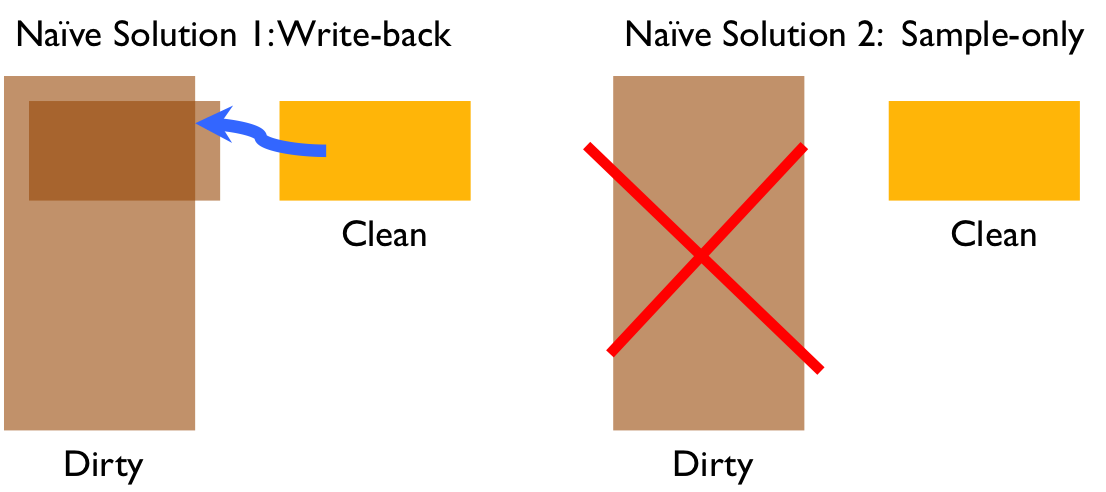
\includegraphics[width=\columnwidth]{figs/update-arch.png}
 \caption{(a) Systematic corruption in one variable can lead to a shifted model. 
 (b) Mixed dirty and clean data results in a less accurate model than no cleaning.
(c) Small samples of only clean data can result in similarly inaccurate models. \label{update-arch-coverletter}}
\end{figure}

\vspace{0.5em}

\noindent\textbf{R1.8 End of Sec 2.1. Why regularization term does not affect the results? It was stated w/o justification.}

\noindent We have revised the paper to make this more clear.
None of the results that we present in this paper depend on the regularization term $r(\theta)$.
Consider the regularized convex-loss minimization problem:
\[
 \theta^{*}=\arg\min_{\theta}\sum_{i=1}^{N}\phi(x_{i},y_{i},\theta) + r(\theta)
\]
Since $r(\theta)$ does not depend on on $i$, we can move it into the sum and treat is as part of $\phi$.
In statistics, the regularization term is required for analysis when ``strong'' convexity is important.


\vspace{0.5em}

\noindent\textbf{R1.9 Example 1 assumes very small sample (50). Why? Is that only for illustration purpose?}

\noindent  A discussion is included in Section \ref{sgd} on why we used 50, and how that value can be set depending on the application. As we noted earlier, sampling is done in iterations. Each iteration samples a batch of 50 records to clean, and this was the batch size used in our experiments. However, the other numbers in the examples (budgets etc.) are chosen for illustration purposes. 

\vspace{0.5em}

\noindent\textbf{R1.9 Sec 4.2. Steps 4-5 need more intuition}

\noindent  We have clarified that Step 4 is a ``is a weighted average of the gradient on the already clean data and newly cleaned data", and Step 5 ``appends the newly cleaned data to set of previously clean records''.

\vspace{0.5em}

\noindent\textbf{R1.10 End of Sec 5. Expected Gradient Length heuristic needs more explanation}

\noindent  The discussion about Expected Gradient Length was an effort to analogize our work with Active Learning, because both are iterative algorithms.  This was a side point that made the text more confusing and we have removed it.
Section \ref{dist-samp} provides a detailed discussion of the sampling problem, what the optimal solution is, and how we apply an approximation to the optimal.

\subsection*{Review 2 Details}

\noindent\textbf{R2.1: Although the problem (iterative data cleaning) is novel, the techniques themselves are quite similar to active learning techniques.}

\noindent  We have included a revised discussion on the differences with Active Learning:

\emph{Active Learning considers the problem of selecting the most informative unlabeled examples to label in partially labeled static data.
Active Learning iteratively queries new examples to label and integrates those examples into the model.
In contrast, we require a broader problem of accounting for modifications to both features and labels in existing examples.
Thus, the data actually changes iteration to iteration.
Furthermore, we have access to dirty values may give us valuable information about which data are likely to be dirty, and which data are likely to impact the model. }

\vspace{0.5em}

\noindent\textbf{R2.2: The selection of the records to clean in each iteration (efficiency problem) uses heuristic solutions (e.g., expected gradient length). There is no formal study of the efficiency of the solution.}

\noindent  As noted in Review 1.10, we apologize for the poor description on our part. We meant to highlight a similarity between \sys and one particular form of Active Learning, and did not intend to imply that we used this approach. 
We have revised the section to make the exact selection procedure clear. Section \ref{det} describes how we partition the data to prioritize data likely to be dirty (not done in Active Learning). Section \ref{dist-samp} formally describes the optimal sampling problem and our solution to it which is an approximation to the optimum. We clearly note that the \sys will convege for any sampling distribution where there is non-zero sampling probability for all remaining dirty records--and more accurate approximations only lead to faster convergence. In all of our experiments, we include \sys+O (ActiveClean + Oracle) which is the theoretical best performance with an optimal sampler and optimal detector.

 \subsection*{Reviewer 3}

\noindent\textbf{R3.1 The background sections were not very clear. This needs to be improved
to make this accessible to a general audience.}

\noindent  We have revised the background section to make the problem more clear. This includes first introducing use cases and the problems with existing tools, and then transitioning to the formalism. We also significantly expanded discussion about the system architecture~(Section \ref{syarch}), which provides intuition on the key insights.

\vspace{0.5em}

\noindent\textbf{R3.2 The jump to sampling over dirty data (Section 5.2) was too abrupt.
I do not understand statistics well enough to see why this will work at all,
and the statistically correct updates argument. Also see D6.}

\noindent  We have made a number of revisions to clarify the relationship between updating, sampling, and detection. We expanded the architecture section to overview the main data flows and an example of how an analyst may use \sys~(Section \ref{syarch}). Section \ref{det} now formalizes and discusses the detection component, and Section \ref{dist-samp} formalizes and discusses the sampling problem.

The main insight of \sys is to model the interactive data cleaning problem as a form of Stochastic Gradient Descent (SGD)~\cite{bottou2012stochastic}.
SGD is an iterative optimization algorithm that starts with an initial estimate and then takes a sequence of steps ``downhill'' to minimize an objective function.
Similarly, in interactive data cleaning, the human starts with a dirty model and makes a series of cleaning decisions to improve the accuracy of the model.
We formalize the link between these two processes, and since SGD is one of the most widely studied forms of optimization, it well understood theoretical convergence conditions.


\vspace{0.5em}

\noindent \textbf{R3.3 I was confused by Identify() in Section 2.4.
From the pseudocode, it appears Identify is picking from R,
those rows that are mispredicted under current\_model.
But why should these be the only rows that are Clean()d.
I thought cleaning was an operation that can
affect both rows that are mispredicted and rows that
are predicted correctly. Update() is not defined.}

\noindent  We have removed the pseudo-code in favor of a more precise discussion of the system architecture in Section \ref{syarch}. This new section highlights all of the components, the key data flows, and their conditions for correctness. 
Additionally, we would like to clarify a point in this review. 
Mispredicted rows are not necessarily dirty data. 
However, poor prediction accuracy might suggest that a record is incorrect, and this would naturally factor in to the selection algorithm of \sys (since those would have a larger gradient).

\vspace{0.5em}

\noindent \textbf{R3.4. Suppose k much less than N .. are retained .. Aren't all
the dirty records cleaned?}

\noindent This section discusses the correctness of the intermeidate result (before the data are fully cleaned).
We meant to say that the user-defined $Clean()$ function was only applied to $k$ records.

\vspace{0.5em}

\noindent\textbf{R3.5. Sentence not clear - ' We have access to direty
values may give us ..'}

 \noindent We have revised this sentence to make it clear. The point that we were trying to make is that Active Learning assumes missing labels, and instead, we assume dirty data. Knowing the dirty value of an attribute (as opposed to it being completely missing) provides valuable information.

\vspace{0.5em}

\noindent\textbf{R3.6. It is not clear where R\_dirty is initialized. Do yu start with R\_dirty -= R? Or is it the set of rows misclassified in the 1st iteration?}

\noindent Section \ref{syarch} now describes the initialization as follows:

\emph{We first set $R_{dirty} = R$ and $R_{clean} = \emptyset$.
The system first trains the model $\phi(\cdot)$ on $R_{dirty}$ to find an initial model $\theta^{(d)}$ that the system will subsequently improve iteratively.
It turns out that SGD converges for an arbitrary initialization, so $\theta^{(d)}$ need not be very accurate. This can be done by featurizing the dirty records (e.g., using an arbitrary placeholder for missing values), and then training the model.}

\vspace{0.5em}

\noindent\textbf{D6. The apriori detector assumption seems bogus.} 

\noindent  We have revised the detector section to be clarify what we meant by the ``a priori'' detector (Section \ref{rule-det}). We have now renamed it a ``rule-based detector'' and have described concrete scenarios in which it applies.

\vspace{0.5em}

\emph{In the data cleaning literature, error detection and error repair are two distinct problems~\cite{DBLP:series/synthesis/2012Fan, Dasu:2003:EDM:861869, rahm2000data}.
Error detection is often considered a substantially easier, since one can often declare a set of integrity rules on a database (e.g., an attribute must not be NULL), and select rows that violate those rules.
On the other hand, repair is harder and often requires human involvement (e.g., imputing a value for the NULL attribute).}

\vspace{0.5em}

\emph{Data quality rules are widely studied as a technique for detecting data errors.
In most rule-based frameworks, an analyst declares a set of rules $\Sigma$ and checks whether a relation $R$ satisfies such rules.
These rules can be declared in advance before applying \sys, or constructed from the first batch of sampled data.
This paper focuses on integrity constraints (ICs), conditional functional dependencies (CFDs), and matching dependencies (MDs) where it is efficient to enumerate the set of records that violate at least one declared rule. }


